%-----------------------------------------------------------------------------------------------
\makeatletter
\immediate\write18{datelog > \jobname.info} % site script for $(date '+%Y-%m-%d %Hh%Mm%Ss')
\makeatother
%-----------------------------------------------------------------------------------------------
%-----------------------------------------------------------------------------------------------
\usetheme{Copenhagen}
\usepackage{beamercolorthemeUTF2}
\usefonttheme{serif}
%-----------------------------------------------------------------------------------------------
\usepackage[utf8]{inputenc}
\usepackage[greek,french,english,brazil]{babel} % last becomes the active one
\usepackage{pslatex}
\usepackage{amssymb,amsmath}
\usepackage{soul}
\usepackage[squaren,Gray,cdot]{SIunits}
\usepackage[nice]{nicefrac}
\usepackage{tikz}
\usepackage{amscd}
\usepackage{stmaryrd}
\usepackage{scalerel}
\usepackage{xspace}
%-----------------------------------------------------------------------------------------------


%-----------------------------------------------------------------------------------------------
%-----------------------------------------------------------------------------------------------
% Mathematical
%-----------------------------------------------------------------------------------------------
\newcommand{\vet}[1]{\underline{{#1}}}
\newcommand{\mat}[1]{\underline{\underline{{#1}}}}
\newcommand{\cub}[1]{\underline{\underline{\underline{{#1}}}}}
\newcommand{\eqdef}{{\ensuremath\stackrel{\text{\tiny def}}{=}}}
%-----------------------------------------------------------------------------------------------
% Linguistic
%-----------------------------------------------------------------------------------------------
\newcommand{\GRtxt}[1]{\begin{otherlanguage}{greek}{{#1}}\end{otherlanguage}}
\newcommand{\FRtxt}[1]{\begin{otherlanguage}{french}{{#1}}\end{otherlanguage}}
%-----------------------------------------------------------------------------------------------
% Presentation
%-----------------------------------------------------------------------------------------------
\newcommand{\BkgImgH}[1]{% Places an image centered on the slide background filling the height
    \usebackgroundtemplate{\parbox{\paperwidth}{%
        \vspace*{1sp}\centering\includegraphics[height=\paperheight]{{#1}}
}}}
\newcommand{\BkgImgW}[1]{% Places an image centered on the slide background filling the width
    \usebackgroundtemplate{\parbox{\paperwidth}{%
        \vspace*{1sp}\centering\includegraphics[width=\paperwidth]{{#1}}
}}}
\newcommand{\ArtEndH}[3]{% Transitions to plain image (last) slide: #1:prefix #2,#3:extensions
    \BkgImgH{root/../art/#1.#2}
    \frame<handout:0>[plain]{%
        \transdissolve\vspace*{72mm}\color{white}\scriptsize\bf\input{root/../art/#1.#3}}
    \usebackgroundtemplate{\mbox{~}}
}
\newcommand{\ArtEndW}[3]{% Transitions to plain image (last) slide: #1:prefix #2,#3:extensions
    \BkgImgW{root/../art/#1.#2}
    \frame<handout:0>[plain]{%
        \transdissolve\vspace*{72mm}\color{white}\scriptsize\bf\input{root/../art/#1.#3}}
    \usebackgroundtemplate{\mbox{~}}
}
\newcommand{\ImgColW}[3]{% Inserts a full-width image in a column
    \includegraphics[width=\columnwidth]{root/../art/#1.#2}\\[-0.5\baselineskip]
    \parbox{\columnwidth}{\tiny\hfill\scalebox{0.85}{\input{root/../art/#1.#3}}}
}
\newcommand{\txtpic}[1]{%
    \fcolorbox{lightgray}{white!90!black}{{#1}} 
}
%-----------------------------------------------------------------------------------------------


%-----------------------------------------------------------------------------------------------
\title{A.03.02 -- Processos Politrópicos}
\subtitle{(Sistemas Fechados)}
\author{Prof.~C.~Naaktgeboren, PhD}
\date{{\scriptsize\tt%
    
\includegraphics[height=6.0mm]{root/00-res/cc/by-nc-nd-88x31.pdf}\\[\smallskipamount]
    https://github.com/CNThermSci/ApplThermSci\\
    Compiled on \input{\jobname.info}
}}
%-----------------------------------------------------------------------------------------------
\begin{document}
%-----------------------------------------------------------------------------------------------
\logo{%
    \parbox{158mm}{% There's a 1mm gap on each side of the 160mm x 90mm slide logo line
        
\includegraphics[height=6.5mm]{root/00-res/UTFPR/UTFPR-logo-A.pdf}\hfill%
        
\includegraphics[height=6.5mm]{root/00-res/logo/CNThermSci-logo-A.pdf}%
%   \parbox{126mm}{% There's a 1mm gap on each side of the 128mm x 96mm slide logo line
%       
\includegraphics[height=6.0mm]{root/00-res/UTFPR/UTFPR-logo-A.pdf}\hfill%
%       
\includegraphics[height=6.0mm]{root/00-res/logo/CNThermSci-logo-A.pdf}%
}} % Alpha logos
%-----------------------------------------------------------------------------------------------
\frame{\titlepage}
%-----------------------------------------------------------------------------------------------

%%-----------------------------------------------------------------------------------------------
%\section*{Sumário Geral}
%%-----------------------------------------------------------------------------------------------
%
%%-----------------------------------------------------------------------------------------------
%\subsection{Parte~I: Apresentação do Trabalho de Fronteira}
%%-----------------------------------------------------------------------------------------------
%
%\frame{
%    \frametitle{Sumário da Parte~I}
%    \tableofcontents[part=1]
%}
%
%%-----------------------------------------------------------------------------------------------
%\subsection{Parte~II: Quantificação do Trabalho de Fronteira}
%%-----------------------------------------------------------------------------------------------
%
%\frame{
%    \frametitle{Sumário da Parte~II}
%    \tableofcontents[part=2]
%}
%
%%===============================================================================================
%\part{Apresentação do Trabalho de Fronteira}
%\frame{\partpage}
%%===============================================================================================

%-----------------------------------------------------------------------------------------------
\section{Apresentação do Trabalho de Fronteira}
%-----------------------------------------------------------------------------------------------

%-----------------------------------------------------------------------------------------------
\subsection{Definição}
%-----------------------------------------------------------------------------------------------

    % !j 96 -i8
    %-------------------------------------------------------------------------------------------
    \begin{frame}{Trabalho de Fronteira -- Definição}\vspace*{-2em}
        \begin{columns}
        \column{0.70\textwidth}
        Trabalho de fronteira, $W_f$ (\kilo\joule)                          \\[\medskipamount]
        \begin{itemize}
            \item É a \alert{interação  energética}                         \\[\medskipamount]
            \item de um \alert{sistema compressível}                        \\[\medskipamount]
            \item capaz de \alert{diretamente} realizar                     \\[\medskipamount]
            \item \alert{trabalho mecânico}                                 \\[\medskipamount]
            \item por meio de uma \alert{fronteira móvel}.
        \end{itemize}
        \column{0.30\textwidth}
        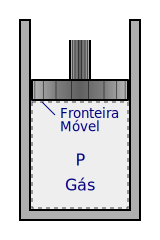
\includegraphics[height=5.0cm]{fig/A0301-pt-VPistCyl.pdf}
        \end{columns}
    \end{frame}
    %-------------------------------------------------------------------------------------------

%-----------------------------------------------------------------------------------------------
\subsection{Aplicações}
%-----------------------------------------------------------------------------------------------

    % !j 96 -i8
    %-------------------------------------------------------------------------------------------
    \begin{frame}<handout>{Trabalho de Fronteira -- Aplicações}\vspace*{-2em}
        \begin{columns}
        \column{0.50\textwidth}
        Aplicações incluem:                                             \\[\medskipamount]
        \begin{itemize}
            \item Motores de combustão interna                          \\[\medskipamount]
            \item Motores \textbf{\alert{Stirling}}                     \\[\medskipamount]
            \item Compressores alternativos                             \\[\medskipamount]
            \item Motores \textbf{\alert{lineares}}                     \\[\medskipamount]
            \item Elevadores de carga e atuadores                       \\[\medskipamount]
            \item Expansores \textbf{\alert{criogênicos}}
        \end{itemize}
        \column{0.15\textwidth}
            \only<1>{\ImgColW{EuroDishSBP_front}{jpg}{txt}}
            \only<2>{\ImgColW{vintage-4273640_1280}{jpg}{txt}}
            \only<3>{\ImgColW{6350734512_4ca40e0711_o}{jpg}{txt}}
        \column{0.35\textwidth}
            \mbox{~}
        \end{columns}
    \end{frame}
    %-------------------------------------------------------------------------------------------

    % !j 96 -i8
    %-------------------------------------------------------------------------------------------
    \begin{frame}<handout:0>{Trabalho de Fronteira -- Aplicações}\vspace*{-2em}
        \begin{columns}
        \column{0.55\textwidth}
        Aplicações incluem: \\[\medskipamount]
        \begin{itemize}
            \item Motores de combustão interna
            \item Motores \textbf{\alert{Stirling}}
        \end{itemize}
        \column{0.45\textwidth}
            \ImgColW{EuroDishSBP_front}{jpg}{txt}
        \end{columns}
    \end{frame}
    %-------------------------------------------------------------------------------------------

    % !j 96 -i8
    %-------------------------------------------------------------------------------------------
    \begin{frame}<handout:0>{Trabalho de Fronteira -- Aplicações}\vspace*{-2em}
        \begin{columns}
        \column{0.55\textwidth}
        Aplicações incluem: \\[\medskipamount]
        \begin{itemize}
            \item Compressores alternativos
            \item Motores \textbf{\alert{lineares}}
        \end{itemize}
        \column{0.45\textwidth}
            \ImgColW{vintage-4273640_1280}{jpg}{txt}
        \end{columns}
    \end{frame}
    %-------------------------------------------------------------------------------------------

    % !j 96 -i8
    %-------------------------------------------------------------------------------------------
    \begin{frame}<handout:0>{Trabalho de Fronteira -- Aplicações}\vspace*{-2em}
        \begin{columns}
        \column{0.55\textwidth}
        Aplicações incluem: \\[\medskipamount]
        \begin{itemize}
            \item Elevadores de carga e atuadores
            \item Expansores \textbf{\alert{criogênicos}}
        \end{itemize}
        \column{0.45\textwidth}
            \ImgColW{6350734512_4ca40e0711_o}{jpg}{txt}
        \end{columns}
    \end{frame}
    %-------------------------------------------------------------------------------------------

%-----------------------------------------------------------------------------------------------
\section{Tópicos de Leitura}
%-----------------------------------------------------------------------------------------------

    %------------------------------------------------------------------------------------------
    \begin{frame}[allowframebreaks]{Tópicos de Leitura}
        \begin{thebibliography}{Çengel, Y.~A., 2013}
            \bibitem[Çengel, Y.~A., 2013]{2013-CengelYA+BolesMA-AMGH}
                Çengel, Y.~A. e Boles, M.~A.
                \newblock{{\em Termodinâmica $7^\mathrm{a}\!$ Edição\/}. \alert{Seção~4-1.}}
                \newblock{\footnotesize AMGH. Porto Alegre. ISBN 978-85-8055-200-3.}
        \end{thebibliography}
    \end{frame}
    %------------------------------------------------------------------------------------------

    % Finishes with stunning image, with credit
    \ArtEndW{horseshoe-bend-1908283_1280}{jpg}{txt}

%===============================================================================================
\part{Quantificação do Trabalho de Fronteira}
\frame{\partpage}
%===============================================================================================

%-----------------------------------------------------------------------------------------------
\section{Quantificação do Trabalho de Fronteira}
%-----------------------------------------------------------------------------------------------

%-----------------------------------------------------------------------------------------------
\subsection{Trabalho de Fronteira De Processo}
%-----------------------------------------------------------------------------------------------

    % !j 96 -i8
    %-------------------------------------------------------------------------------------------
    \begin{frame}{Trabalho de Fronteira -- Diferencial}\vspace*{-2em}
        \begin{columns}
        \column{0.55\textwidth}
            \begin{align*}
                \uncover<1->{%
                    \delta W_f & \equiv
                    \uncover<2->{(|}\vec{F}\uncover<2->{|} \cdot \uncover<2->{|}d\vec\ell
                    \uncover<2->{|)\times\frac{A}{A}\rightharpoondown} \\}
                \uncover<3->{%
                    \delta W_f & = \frac{F}{A} \cdot A\,d\ell
                    \rightharpoondown \\[\medskipamount]}
                \uncover<4->{%
                    \biggl(
                        \frac{F}{A} & \equiv P,\quad
                        A\,d\ell      \equiv dV
                    \biggr) \rightharpoondown \\[\medskipamount]}
                \uncover<5->{%
                    \uncover<6->{(} \delta W_f & = P\,dV
                    \uncover<6->{)/m \rightharpoondown} \\[\medskipamount]}
                \uncover<7->{%
                    \delta w_f & = P\,dv }
            \end{align*}
        \column{0.45\textwidth}
            $W_f > 0$ quando o \alert{sistema executa} trabalho
            \begin{figure}
                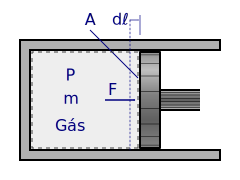
\includegraphics[width=5.0cm]{fig/A0301-pt-HPistCyl.pdf}
            \end{figure}
        \end{columns}
    \end{frame}
    %-------------------------------------------------------------------------------------------

    % !j 96 -i8
    %-------------------------------------------------------------------------------------------
    \begin{frame}{Trabalho de Fronteira -- Processo}\vspace*{-2em}
        \begin{columns}
        \column{0.55\textwidth}
            Processo de \alert{quase-equilíbrio} $1$--$2$:
            \begin{align*}
                \uncover<1->{%
                    \delta w_f & = P\,dv \\[\medskipamount]}
                \uncover<2->{%
                    \uncover<3->{\biggl(}
                        w_{12} & = \int_1^2 \delta w_f = \int_1^2 P\,dv
                    \uncover<3->{\biggr)\times m \rightharpoondown} \\[\medskipamount]}
                \uncover<4->{%
                    W_{12} & = \int_1^2 \delta W_f = \int_1^2 P\,dV
                    \uncover<5->{\quad\therefore}}
            \end{align*}
            \uncover<6->{$W_f$ é a \alert{área} sob o processo em \alert{coordenadas $P-V$}.}\\
            \uncover<7->{$w_f$ é a \alert{área} sob o processo em \alert{coordenadas $P-v$}.}
        \column{0.45\textwidth}
            \begin{figure}
                \alt<1-5>%
                    {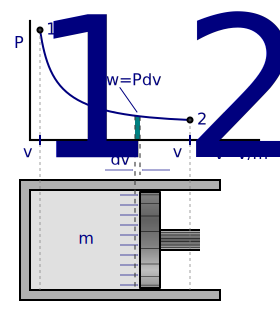
\includegraphics[width=5.0cm]{fig/A0301-pt-HPistCylPlot.pdf}}
                    {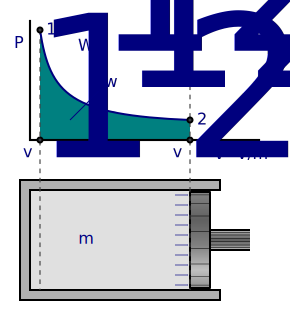
\includegraphics[width=5.0cm]{fig/A0301-pt-HPistCylPlotInt.pdf}}
            \end{figure}
        \end{columns}
    \end{frame}
    %-------------------------------------------------------------------------------------------

    % !j 96 -i8
    %-------------------------------------------------------------------------------------------
    \begin{frame}{Trabalho de Fronteira -- Caminho}\vspace*{-2em}
        \begin{columns}
        \column{0.55\textwidth}
        Trabalho de fronteira, $w_f$ ou $W_f$:
        \begin{itemize}
            \item<1-> Depende do \alert{caminho $1$--$2$} \\[\medskipamount]
            \item<2-> $\int_1^2\delta w_f = w_{12}\;$\uncover<3->{\alert{$\neq
                \mbox{``}w_2\mbox{''} - \mbox{``}w_1\mbox{''}$}} \\[\medskipamount]
            \item<4-> A \alert{diferença} entre caminhos é determinada pelas demais interações
                de energia durante o processo $1$--$2$ \\[\medskipamount]
            \item<5-> Em \alert{sistemas compressíveis simples}, o \alert{calor} é a única outra
                interação de energia.
        \end{itemize}
        \column{0.45\textwidth}
            \begin{figure}
                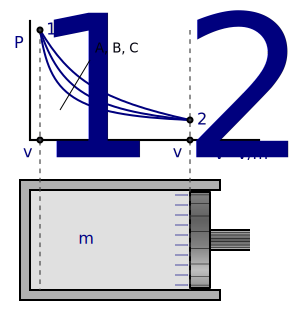
\includegraphics[width=5.0cm]{fig/A0301-pt-HPistCylPlotPath.pdf}
            \end{figure}
        \end{columns}
    \end{frame}
    %-------------------------------------------------------------------------------------------

%-----------------------------------------------------------------------------------------------
\subsection{Trabalho de Fronteira de Ciclo}
%-----------------------------------------------------------------------------------------------

    % !j 96 -i8
    %-------------------------------------------------------------------------------------------
    \begin{frame}{Trabalho de Fronteira -- Ciclo}\vspace*{-2em}
        \begin{columns}
        \column{0.55\textwidth}
        \begin{itemize}
            \small
            \item<1-> A dependência do caminho permite que um sistema executando um vai-vém
                (\alert{ciclo mecânico}) possa tanto (i)~produzir ou (ii)~consumir uma
                quantidade \alert{líquida} de trabalho. \\[\medskipamount]
            \item<2-> Basta escolher os caminhos de ida e volta no processo termodinâmico.
                \\[\medskipamount]
            \item<3-> Se os \alert{estados} periodicamente visitados pelo sistema forem
                \alert{os mesmos}, o sistema estará executando um \alert{ciclo termodinâmico}.
        \end{itemize}
        \column{0.45\textwidth}
            \begin{figure}
                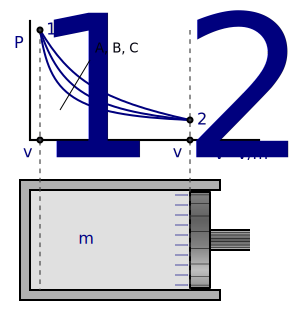
\includegraphics[width=5.0cm]{fig/A0301-pt-HPistCylPlotPath.pdf}
            \end{figure}
        \end{columns}
    \end{frame}
    %-------------------------------------------------------------------------------------------

    % !j 96 -i8
    %-------------------------------------------------------------------------------------------
    \begin{frame}{Trabalho de Fronteira -- Ciclo}\vspace*{-2em}
        \begin{columns}
        \column{0.55\textwidth}
        Ciclo $1$--$2$ via `C' e $2$--$1$ via `A':
        \begin{itemize}
            \item<1> Ciclo \alert{motor}, que \alert{produz} $W_{liq}$
            \item<0> $W_{acum}$ mostrado sob os processos
            \item<0> Exp.~$1$--$2$ \alert{produz} trabalho $W_{12} > 0$
            \item<0> Retorno ao estado $1$ requer \alert{consumo} de trabalho
            \item<0> Compr.~$2$--$1$ \alert{produz} trabalho $W_{21} < 0$
            \item<0> $W_{\mathrm{ciclo}} = (W_{12} + W_{21}) > 0$ é igual à \alert{área do
                ciclo} em \alert{coordenadas $P-V$}.
        \end{itemize}
        \column{0.45\textwidth}
            \begin{figure}
                \only<1>{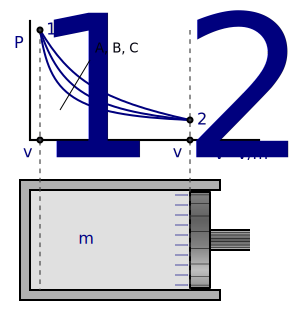
\includegraphics[width=5.0cm]{fig/A0301-pt-HPistCylPlotPath.pdf}}
               %\only<1>{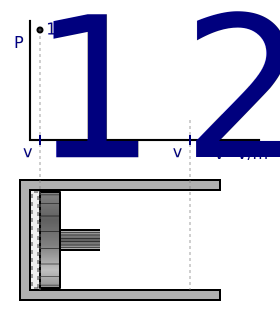
\includegraphics[width=5.0cm]{fig/A0301-pt-HPistCylPlotCycle-00.pdf}}
               %\only<1>{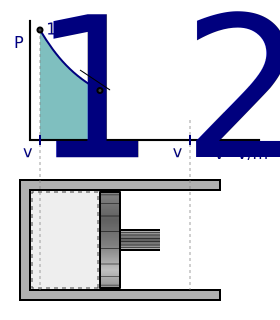
\includegraphics[width=5.0cm]{fig/A0301-pt-HPistCylPlotCycle-01.pdf}}
               %\only<1>{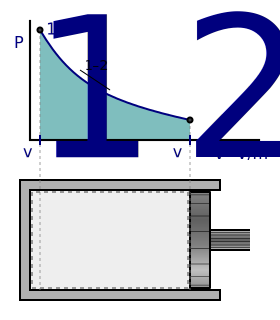
\includegraphics[width=5.0cm]{fig/A0301-pt-HPistCylPlotCycle-02.pdf}}
               %\only<1>{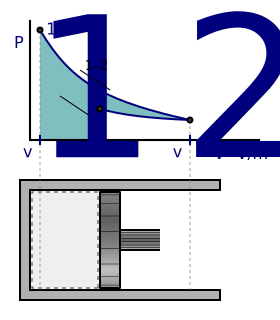
\includegraphics[width=5.0cm]{fig/A0301-pt-HPistCylPlotCycle-03.pdf}}
               %\only<1>{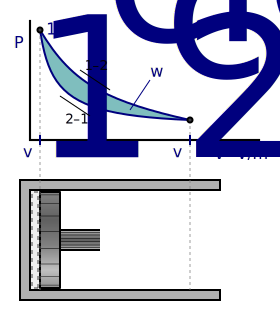
\includegraphics[width=5.0cm]{fig/A0301-pt-HPistCylPlotCycle-05.pdf}}
            \end{figure}
        \end{columns}
    \end{frame}
    %-------------------------------------------------------------------------------------------
    \begin{frame}<handout:0>{Trabalho de Fronteira -- Ciclo}\vspace*{-2em}
        \begin{columns}
        \column{0.55\textwidth}
        Ciclo $1$--$2$ via `C' e $2$--$1$ via `A':
        \begin{itemize}
            \item<1> Ciclo \alert{motor}, que \alert{produz} $W_{liq}$
            \item<1> $W_{acum}$ mostrado sob os processos
            \item<0> Exp.~$1$--$2$ \alert{produz} trabalho $W_{12} > 0$
            \item<0> Retorno ao estado $1$ requer \alert{consumo} de trabalho
            \item<0> Compr.~$2$--$1$ \alert{produz} trabalho $W_{21} < 0$
            \item<0> $W_{\mathrm{ciclo}} = (W_{12} + W_{21}) > 0$ é igual à \alert{área do
                ciclo} em \alert{coordenadas $P-V$}.
        \end{itemize}
        \column{0.45\textwidth}
            \begin{figure}
               %\only<1>{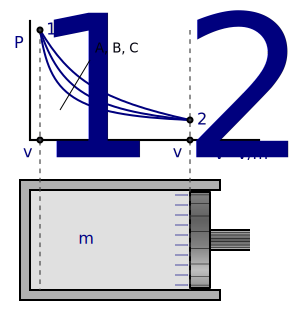
\includegraphics[width=5.0cm]{fig/A0301-pt-HPistCylPlotPath.pdf}}
                \only<1>{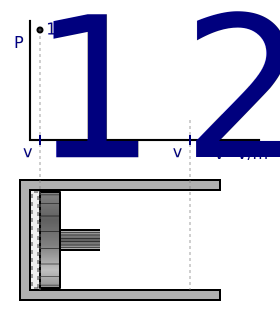
\includegraphics[width=5.0cm]{fig/A0301-pt-HPistCylPlotCycle-00.pdf}}
               %\only<1>{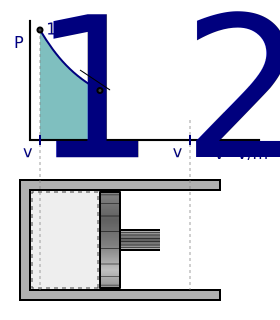
\includegraphics[width=5.0cm]{fig/A0301-pt-HPistCylPlotCycle-01.pdf}}
               %\only<1>{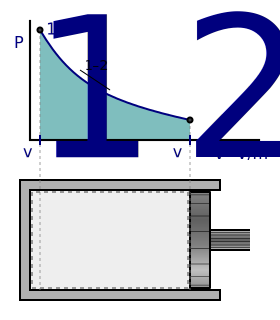
\includegraphics[width=5.0cm]{fig/A0301-pt-HPistCylPlotCycle-02.pdf}}
               %\only<1>{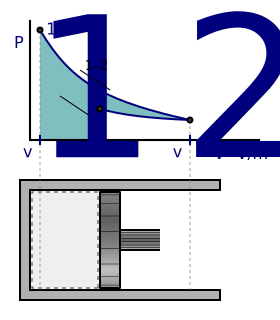
\includegraphics[width=5.0cm]{fig/A0301-pt-HPistCylPlotCycle-03.pdf}}
               %\only<1>{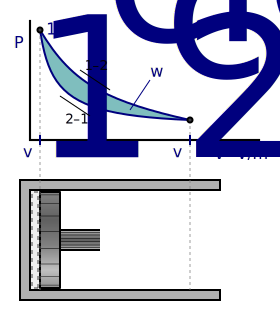
\includegraphics[width=5.0cm]{fig/A0301-pt-HPistCylPlotCycle-05.pdf}}
            \end{figure}
        \end{columns}
    \end{frame}
    %-------------------------------------------------------------------------------------------
    \begin{frame}<handout:0>{Trabalho de Fronteira -- Ciclo}\vspace*{-2em}
        \begin{columns}
        \column{0.55\textwidth}
        Ciclo $1$--$2$ via `C' e $2$--$1$ via `A':
        \begin{itemize}
            \item<1> Ciclo \alert{motor}, que \alert{produz} $W_{liq}$
            \item<1> $W_{acum}$ mostrado sob os processos
            \item<1> Exp.~$1$--$2$ \alert{produz} trabalho $W_{12} > 0$
            \item<0> Retorno ao estado $1$ requer \alert{consumo} de trabalho
            \item<0> Compr.~$2$--$1$ \alert{produz} trabalho $W_{21} < 0$
            \item<0> $W_{\mathrm{ciclo}} = (W_{12} + W_{21}) > 0$ é igual à \alert{área do
                ciclo} em \alert{coordenadas $P-V$}.
        \end{itemize}
        \column{0.45\textwidth}
            \begin{figure}
               %\only<1>{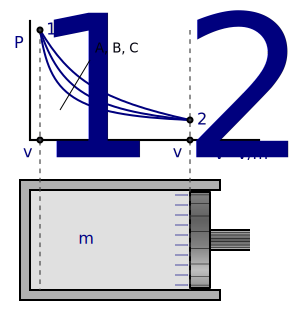
\includegraphics[width=5.0cm]{fig/A0301-pt-HPistCylPlotPath.pdf}}
               %\only<1>{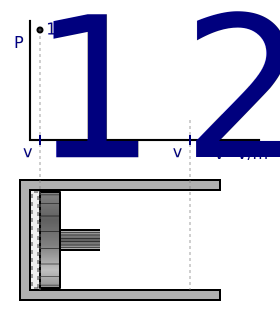
\includegraphics[width=5.0cm]{fig/A0301-pt-HPistCylPlotCycle-00.pdf}}
                \only<1>{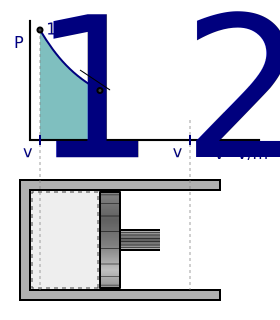
\includegraphics[width=5.0cm]{fig/A0301-pt-HPistCylPlotCycle-01.pdf}}
               %\only<1>{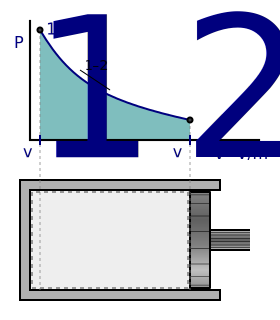
\includegraphics[width=5.0cm]{fig/A0301-pt-HPistCylPlotCycle-02.pdf}}
               %\only<1>{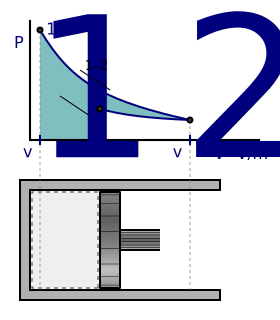
\includegraphics[width=5.0cm]{fig/A0301-pt-HPistCylPlotCycle-03.pdf}}
               %\only<1>{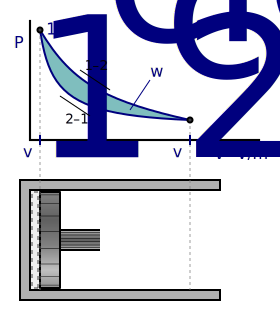
\includegraphics[width=5.0cm]{fig/A0301-pt-HPistCylPlotCycle-05.pdf}}
            \end{figure}
        \end{columns}
    \end{frame}
    %-------------------------------------------------------------------------------------------
    \begin{frame}<handout:0>{Trabalho de Fronteira -- Ciclo}\vspace*{-2em}
        \begin{columns}
        \column{0.55\textwidth}
        Ciclo $1$--$2$ via `C' e $2$--$1$ via `A':
        \begin{itemize}
            \item<1> Ciclo \alert{motor}, que \alert{produz} $W_{liq}$
            \item<1> $W_{acum}$ mostrado sob os processos
            \item<1> Exp.~$1$--$2$ \alert{produz} trabalho $W_{12} > 0$
            \item<1> Retorno ao estado $1$ requer \alert{consumo} de trabalho
            \item<0> Compr.~$2$--$1$ \alert{produz} trabalho $W_{21} < 0$
            \item<0> $W_{\mathrm{ciclo}} = (W_{12} + W_{21}) > 0$ é igual à \alert{área do
                ciclo} em \alert{coordenadas $P-V$}.
        \end{itemize}
        \column{0.45\textwidth}
            \begin{figure}
               %\only<1>{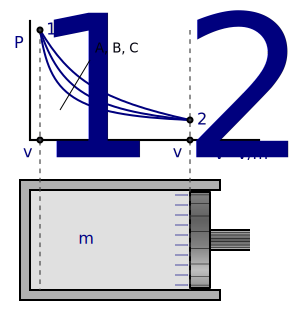
\includegraphics[width=5.0cm]{fig/A0301-pt-HPistCylPlotPath.pdf}}
               %\only<1>{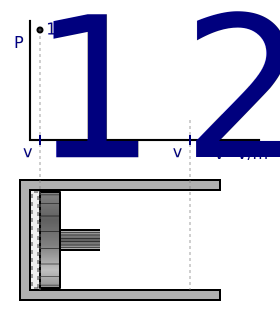
\includegraphics[width=5.0cm]{fig/A0301-pt-HPistCylPlotCycle-00.pdf}}
               %\only<1>{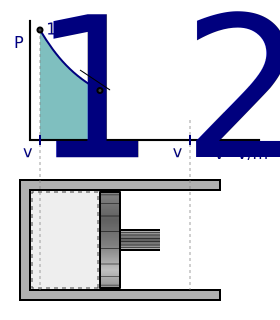
\includegraphics[width=5.0cm]{fig/A0301-pt-HPistCylPlotCycle-01.pdf}}
                \only<1>{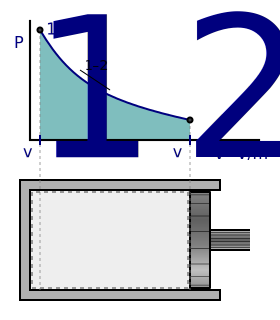
\includegraphics[width=5.0cm]{fig/A0301-pt-HPistCylPlotCycle-02.pdf}}
               %\only<1>{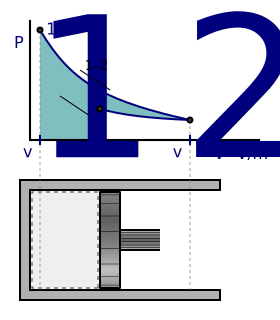
\includegraphics[width=5.0cm]{fig/A0301-pt-HPistCylPlotCycle-03.pdf}}
               %\only<1>{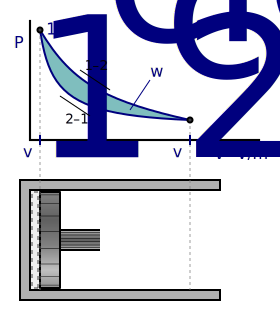
\includegraphics[width=5.0cm]{fig/A0301-pt-HPistCylPlotCycle-05.pdf}}
            \end{figure}
        \end{columns}
    \end{frame}
    %-------------------------------------------------------------------------------------------
    \begin{frame}<handout:0>{Trabalho de Fronteira -- Ciclo}\vspace*{-2em}
        \begin{columns}
        \column{0.55\textwidth}
        Ciclo $1$--$2$ via `C' e $2$--$1$ via `A':
        \begin{itemize}
            \item<1> Ciclo \alert{motor}, que \alert{produz} $W_{liq}$
            \item<1> $W_{acum}$ mostrado sob os processos
            \item<1> Exp.~$1$--$2$ \alert{produz} trabalho $W_{12} > 0$
            \item<1> Retorno ao estado $1$ requer \alert{consumo} de trabalho
            \item<1> Compr.~$2$--$1$ \alert{produz} trabalho $W_{21} < 0$
            \item<0> $W_{\mathrm{ciclo}} = (W_{12} + W_{21}) > 0$ é igual à \alert{área do
                ciclo} em \alert{coordenadas $P-V$}.
        \end{itemize}
        \column{0.45\textwidth}
            \begin{figure}
               %\only<1>{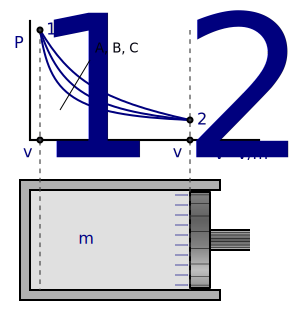
\includegraphics[width=5.0cm]{fig/A0301-pt-HPistCylPlotPath.pdf}}
               %\only<1>{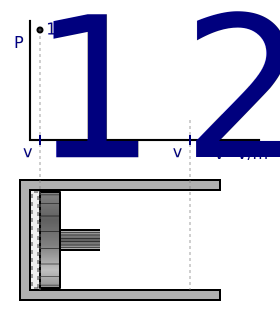
\includegraphics[width=5.0cm]{fig/A0301-pt-HPistCylPlotCycle-00.pdf}}
               %\only<1>{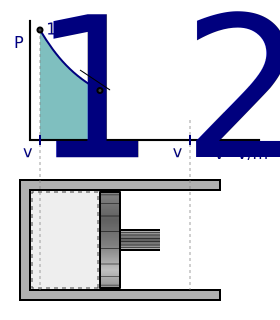
\includegraphics[width=5.0cm]{fig/A0301-pt-HPistCylPlotCycle-01.pdf}}
               %\only<1>{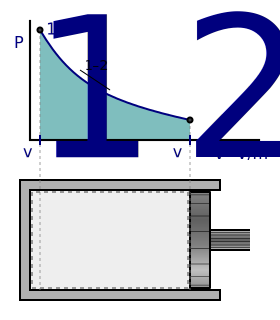
\includegraphics[width=5.0cm]{fig/A0301-pt-HPistCylPlotCycle-02.pdf}}
                \only<1>{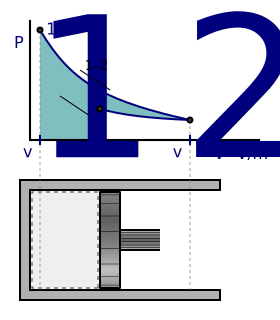
\includegraphics[width=5.0cm]{fig/A0301-pt-HPistCylPlotCycle-03.pdf}}
               %\only<1>{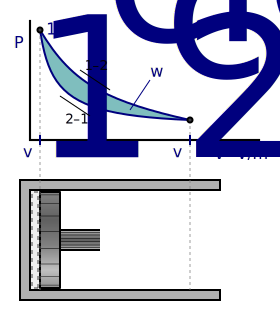
\includegraphics[width=5.0cm]{fig/A0301-pt-HPistCylPlotCycle-05.pdf}}
            \end{figure}
        \end{columns}
    \end{frame}
    %-------------------------------------------------------------------------------------------
    \begin{frame}{Trabalho de Fronteira -- Ciclo}\vspace*{-2em}
        \begin{columns}
        \column{0.55\textwidth}
        Ciclo $1$--$2$ via `C' e $2$--$1$ via `A':
        \begin{itemize}
            \item<1> Ciclo \alert{motor}, que \alert{produz} $W_{liq}$
            \item<1> $W_{acum}$ mostrado sob os processos
            \item<1> Exp.~$1$--$2$ \alert{produz} trabalho $W_{12} > 0$
            \item<1> Retorno ao estado $1$ requer \alert{consumo} de trabalho
            \item<1> Compr.~$2$--$1$ \alert{produz} trabalho $W_{21} < 0$
            \item<1> $W_{\mathrm{ciclo}} = (W_{12} + W_{21}) > 0$ é igual à \alert{área do
                ciclo} em \alert{coordenadas $P-V$}.
        \end{itemize}
        \column{0.45\textwidth}
            \begin{figure}
               %\only<1>{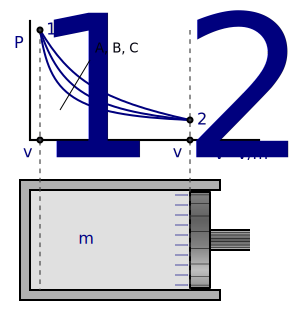
\includegraphics[width=5.0cm]{fig/A0301-pt-HPistCylPlotPath.pdf}}
               %\only<1>{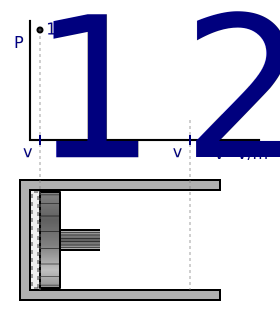
\includegraphics[width=5.0cm]{fig/A0301-pt-HPistCylPlotCycle-00.pdf}}
               %\only<1>{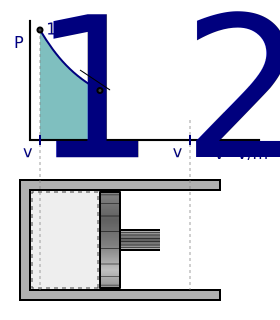
\includegraphics[width=5.0cm]{fig/A0301-pt-HPistCylPlotCycle-01.pdf}}
               %\only<1>{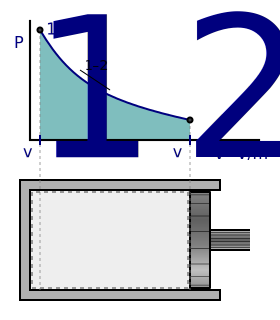
\includegraphics[width=5.0cm]{fig/A0301-pt-HPistCylPlotCycle-02.pdf}}
               %\only<1>{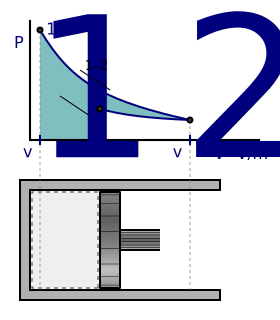
\includegraphics[width=5.0cm]{fig/A0301-pt-HPistCylPlotCycle-03.pdf}}
                \only<1>{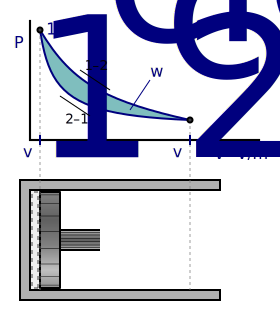
\includegraphics[width=5.0cm]{fig/A0301-pt-HPistCylPlotCycle-05.pdf}}
            \end{figure}
        \end{columns}
    \end{frame}
    %-------------------------------------------------------------------------------------------

%-----------------------------------------------------------------------------------------------
\section{Tópicos de Leitura}
%-----------------------------------------------------------------------------------------------

    %------------------------------------------------------------------------------------------
    \begin{frame}[allowframebreaks]{Tópicos de Leitura}
        \begin{thebibliography}{Çengel, Y.~A., 2013}
            \bibitem[Çengel, Y.~A., 2013]{2013-CengelYA+BolesMA-AMGH}
                Çengel, Y.~A. e Boles, M.~A.
                \newblock{{\em Termodinâmica $7^\mathrm{a}\!$ Edição\/}. \alert{Seção~4-1.}}
                \newblock{\footnotesize AMGH. Porto Alegre. ISBN 978-85-8055-200-3.}
        \end{thebibliography}
    \end{frame}
    %------------------------------------------------------------------------------------------

    % Finishes with stunning image, with credit
    \ArtEndW{tree-4503535_1280}{jpg}{txt}

%-----------------------------------------------------------------------------------------------
\end{document}
%-----------------------------------------------------------------------------------------------

